\documentclass[thesis.tex]{subfiles}

\begin{document}

\chapter{Prerequisite concepts}

In this section I introduce some basic concepts needed to understand the appended research papers. 

\section{Forces on particles in fluids}\label{sec:forces}

We are studying the dynamics of small particles suspended in flows.
Specifically, we consider particles small enough to not create disturbances in the fluid flow. In such cases, one can consider the fluid flow as a prescribed input, and calculate the response of the particles. 
What I mean is that the particle does not induce long-lived disturbances in the fluid, which survive to affect the particle at a later time. In order to understand this requirement, and how the particle forces are calculated, we start at the Navier-Stokes equation.

The governing equation for an incompressible, Newtonian fluid is the Navier-Stokes equation
\begin{align}
	\rho_f \left(\frac{\partial}{\partial t}\ve u + \ve u \cdot \nabla \ve u\right) &= -\nabla p + \mu \nabla^2 \ve u, \eqnlab{navierstokes}
\intertext{with the incompressibility condition}
	\nabla \cdot \ve u &= 0. \nn
\end{align}
Here $\rho_f$ is the density of the fluid, which by the incompressibility condition is assumed to be the same everywhere. The vector field $\ve u(\ve x, t)$ is the fluid velocity, defined at all points in space, and $p(\ve x, t)$ is the scalar pressure field, also defined at all points in space. The parameter $\mu$ is the dynamic viscosity of the fluid, which by definition is the relation between stress and strain in a Newtonian fluid. Sometimes we instead use the kinematic viscosity $\nu = \mu/\rho_f$. The definition of a Newtonian fluid is that the viscosity is constant. One commonly used boundary condition to \Eqnref{navierstokes} is the no-slip condition, meaning zero relative velocity between the boundary and the fluid.

We will often, especially when discussing the orientational dynamics of particles, encounter the fluid flow gradient $\ma A = \nabla \ve u\transpose$, or on component form
\begin{align*}
	A_{ij} &= \frac{\partial u_i}{\partial x_j}.
\end{align*}
The incompressibility condition $\nabla\cdot\ve u=0$ transfers directly to the condition $\tr \ma A=0$.

Throughout this thesis I employ the implicity summation convention for repeated indices. The implied summation is over the number of spatial degrees of freedom, for example
\begin{align*}
	A_{ii} = \sum_{i=1}^d A_{ii} = \tr \ma A.
\end{align*}

The gradient $\ma A$ is often split into its symmetric and anti-symmetric parts such that
\begin{align*}
	&\ma O = \frac{1}{2}(\ma A - \ma A\transpose),\quad
	\ma S = \frac{1}{2}(\ma A + \ma A\transpose),\quad
	\ma A = \ma O + \ma S.
\end{align*}
The symmetric part $\ma S$ is called the rate-of-strain tensor, and it contains the local rate of deformation of the flow. The anti-symmetric part $\ma O$ is related to the vorticity vector. The vorticity vector $\ve \omega_f$ of a flow $\ve u$ is defined by $\ve \omega_f = \nabla \cross \ve u$. The matrix $\ma O$ is related to the vorticity vector $\ve \omega_f$, because for any given vector $\ve x$
\begin{align}
	\ma O \ve x &= \frac{1}{2}\ve \omega_f \cross \ve x \equiv \ve \Omega \cross \ve x.\eqnlab{vorticityOdef}
\end{align}
The vector $\ve \Omega$, defined as half the vorticity, is a common quantitiy in our calculations, and therefore is given its own symbol. Expressed in index notation the elements of $\ma O$ are related to $\ve \Omega$ by $O_{ij} = -\lc_{ijp}\Omega_p$. Here and in this thesis $\lc$ denotes the anti-symmetric third order tensor
\begin{align*}
\lc_{ijk} = \begin{cases}
+1 & \textrm{if } (i,j,k) \textrm{ is a cyclic permutation of} (1,2,3), \\
-1 & \textrm{if } (i,j,k) \textrm{ is a cyclic permutation of } (3,2,1), \\
\;\;\,0 & \textrm{if two indices are equal.}
\end{cases}\end{align*}

The stress tensor $\ma T$ of a fluid is a symmetric second order tensor defined at each point in space. Its elements $T_{ij}$ are defined as the $i$:th component of the force on a surface with (outward pointing) normal in the $j$:th direction. That is, if a surface has outward normal $\ve n$, the force $\ve f$ per unit area is
\begin{align*}
	\ve f &= \ma T \ve n.
\end{align*}
Due to this interpretation, the diagonal elements of $\ma T$ are called normal stresses, and the off-diagonal elements shear stresses. For an incompressible and Newtonian fluid the stress tensor is
\begin{align*}
	\ma T &= -p \ma I + 2\mu \ma S,
\end{align*}
where $\ma I$ denotes the identity tensor. This relation is not a result, as much as part of the definition of Newtonian fluids. The relation is in fact used in the derivation of the Navier-Stokes equation \eqnref{navierstokes} \cite{kundu2004}. 

There are two steps to compute the force on a particle suspended in the fluid. First one has to solve the Navier-Stokes equation, with the particle as a boundary. Then one must integrate the resulting stress tensor over the entire particle surface. The Navier-Stokes equation \eqnref{navierstokes} contains non-linear terms, and does not, in general, admit an analytical solution. We may understand that the problem is very hard just by imagining a particle in a fluid: as the particle moves and rotates, it stirs up a wake and vortices in its trail. These disturbances may linger and affect the particle at a later time. It seems that we are, in general, obliged to take into account the whole joint history of the particle and the fluid to predict the final state of the two.

But if the particle is sufficiently small, the disturbances will be smeared out by the viscous forces before they make any secondary impact. The condition is precisely that the particle Reynolds number is small. As stated in Sec.~\ref{sec:context},
\begin{align*}
 	\rep = \frac{\textrm{Viscous time}}{\textrm{Time for fluid to flow one particle length}}.
\end{align*}
More specifically,
\begin{align*}
	\rep = \frac{u_0 a}{\nu},
\end{align*}
where $u_0$ is a typical flow speed relative to the particle surface, $a$ is the size of the particle and $\nu$ is the kinematic viscosity of the fluid. In the extreme case when $\rep=0$, the Navier-Stokes equation \eqnref{navierstokes} reduces to the linear steady Stokes equation \cite{kim1991,kundu2004}
\begin{align*}
	\mu \nabla^2 \ve u = \nabla p.
\end{align*}
This type of flow condition is called viscous flow, or creeping flow. Because the governing equation is linear, many more problems admit analytical solutions. In particular, the force and torque on a particle in viscous flow has been worked out in quite some detail. The formalism of resistance tensors was introduced by Brenner \cite{brenner1974, happel1965}, but here I follow the notation used in the book \emph{Microhydrodynamics} by Kim \& Karrila \cite{kim1991}.

The fundamental result is that the force and torque on a particle suspended in a flow is linearly related to the undisturbed flow. Given the particle velocity $\ve v$ and angular velocity $\ve \omega$, we write the force $\ve F$ and torque $\ve T$ as
\begin{align}
	\ve F &= \te A (\ve u - \ve v) + \te B (\ve \Omega - \ve \omega), \nn \\
	\ve T &= \te B\transpose (\ve u - \ve v) + \te C (\ve \Omega - \ve \omega) + \te H \dd \ma S. \eqnlab{resistanceformulation}
\end{align}
The resistance tensors $\te A$, $\te B$, $\te C$ and $\te H$ depend only upon particle shape, and can be computed once and for all. The tensor $\te H$ is third order, and the double dot product $\te H \dd \ma S$ is a contraction over two indices. In index notation it reads $(\te H \dd \ma S)_i = H_{ijk}S_{jk}$. 

The resistance tensors in the case of a sphere of radius $a$ are  $\te A = 6\pi\mu a \ma I$, $\te B=\te H = 0$ and $\te C = 8\pi\mu a^3 \ma I$. In fact, for any particle which is mirror-symmetric in all three cartesian planes it holds that $\te B = 0$. In such cases there is neither coupling between rotation and force, nor between translation and torque. 

For non-spherical particles there is a hidden complication in \Eqnref{resistanceformulation}: the flow is usually known in a fixed frame of reference, but the resistance tensors are known in the frame of reference of the particle. Expressing the resistance tensors in the fixed frame of reference entails a rotation dependent on the particle orientation. Thus, the torque is in general a non-linear function of particle orientation.

The hydrodynamic resistance of an ellipsoid was computed in a now famous paper by Jeffery in 1922 \cite{jeffery1922}. The result therein is of course not expressed in the subsequently invented tensor notation, but all the necessary calculations are there. The adaptation to current notation is found in \emph{Microhydrodynamics} (Ref.~\citenum{kim1991} p.~56). All calculations in this thesis, and the appended papers, proceed from forces and torques obtained in this manner. Therefore the assumption of $\rep = 0$ is implicit everywhere, even if not explicitly stated.

When the force and torque on a particle are known, its trajectory is determined by Newton's equations of motion for a rigid body. Since the torque may depend non-linearly upon particle orientation, solving the rigid-body equations is in general not possible. The first approximation, introduced already by Jeffery in 1922, is the over-damped limit where particle inertia is neglected. The resulting equation of motion is discussed in Sec.~\ref{sec:jefferyequation}, but first we will discuss the anatomy of the simple shear flow in Sec.~\ref{sec:shearflow}.

\section{Simple shear flow}\label{sec:shearflow}

The simple shear flow is a uni-directional linear flow which varies magnitude in only one transversal direction. It is shown in Fig.~\ref{fig:shear_decomposition}. The equation describing the shear flow is simply,
\begin{align*}
	\ve u(y) &= s y \hat{\ve x}.
\end{align*}
Here $s$ is a scalar called the shear strength, and $y$ is the coordinate along the $\hat{\ve y}$-axis. 
Fig.~\ref{fig:coordinates} shows the coordinate system we use for shear flows in this thesis and in the appended papers. The three principal directions are the flow direction $\hat{\ve x}$, the shear direction $\hat{\ve y}$ and the vorticity direction $\hat{\ve z}$. The vorticity direction $\hat{\ve z}$ is also the direction of $\ve \Omega$ introduced in Sec.~\ref{sec:forces}.

The flow gradient of the simple shear flow is constant and given by
\begin{align*}
	\ma A = \begin{bmatrix}
		0 & s & 0 \\
		0 & 0 & 0 \\
		0 & 0 & 0 
	\end{bmatrix}.
\end{align*}
The shear flow is important for two reasons. First, it is one of the fundamental flows in rheology, the study of fluids. It is the flow inside a Couette device, used for example to measure viscosity. Second, as far as particle dynamics go, the simple shear flow is relevant for \emph{any} flow with parallel streamlines. Consider for example the flow of a suspension through a pipe. The pipe is assumed to be large compared to the suspended particles, and the flow profile is most likely a complicated function of position $y$ in the pipe cross section\footnote{In principle the function should also depend on the position in the $z$-direction. In that case the result is also a simple shear flow, although rotated.}:
\begin{align*}
	\ve u(y) &= f(y)\hat{\ve x},
\end{align*}
 and the flow gradient is
\begin{align*}
	\ma A = \begin{bmatrix}
		0 & f'(y) & 0 \\
		0 & 0 & 0 \\
		0 & 0 & 0 
	\end{bmatrix}.
\end{align*}
Thus, if the flow profile $f$ varies slowly over the particle size, the particle experiences a simple shear flow of strength $f'(y)$. This is exactly the case in the experiment described in Paper A (see \Secref{experiment}).

Curiously, the dynamics of non-spherical particles in simple shear flow offers a rich variety of behaviours. There is no stationary state, but a particle tumbles end-to-end indefinitely. If the particle is axisymmetric, the tumbling is periodic. The technical details and explanations of this are discussed in Sec.~\ref{sec:jefferyequation}, but we can understand the underlying reason from the composition of the shear flow. Fig.~\ref{fig:shear_decomposition} illustrates schematically how the shear is a superposition of two flows. One is a pure rotation, corresponding to the antisymmetric part $\ma O$ of the flow gradient. The other is a pure strain, the symmetric part $\ma S$ of the flow gradient. Now imagine a rod-shaped particle in these flows. The pure rotation, the vorticity, will rotate the rod with a constant angular velocity, regardless of the rod's orientation. The strain, on the other hand, has a preferred direction to which it will attract the long axis of the rod. Sometimes the vorticity and strain will cooperate to turn the rod onto the strain eigendirection, and sometimes the vorticity will struggle to rotate the rod out of the attracting direction. The result is that the rod will always rotate, but sometimes faster and sometimes slower. When the difference between the fast and the slow rotations is large, we perceive this as intermittent tumbling.
\begin{figure}
\begin{center}
%  \makebox[\textwidth]{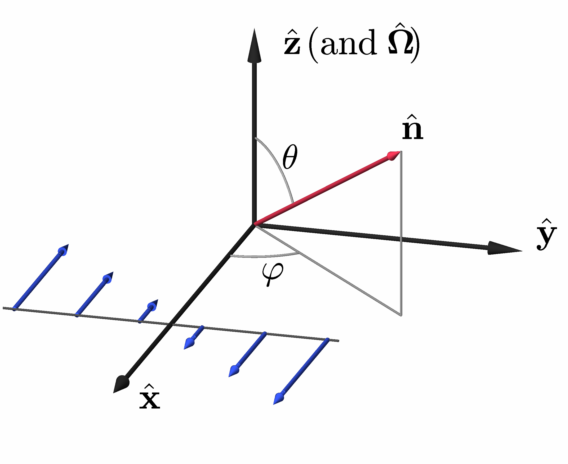
\includegraphics[width=7cm]{figs/fig_coordinates.png}}
\begin{lpic}{figs/fig_coordinates(7cm,)}
   \lbl[tl]{40,9;$\hat{\ve x}$}
   \lbl[tl]{140,45;$\hat{\ve y}$}
   \lbl[tl]{80,115;$\hat{\ve z}$}
   \lbl[bl]{120,80;$\ve n$}
   \lbl[bl]{85,75;$\theta$}
   \lbl[tl]{75,45;$\varphi$}
\end{lpic}
\end{center}
\caption{\figlab{coordinates}Coordinate system of simple shear flow in this thesis. The same system is used in Papers A \& B. The directions are the flow direction $\hat{\ve x}$, the shear direction $\hat{\ve y}$, and the vorticity direction $\hat{\ve z}$. The angles $(\theta, \varphi)$ are the spherical coordinates of the particle direction vector $\ve n$. }%
\end{figure}
\begin{figure}
\begin{center}
  %\makebox[\textwidth]{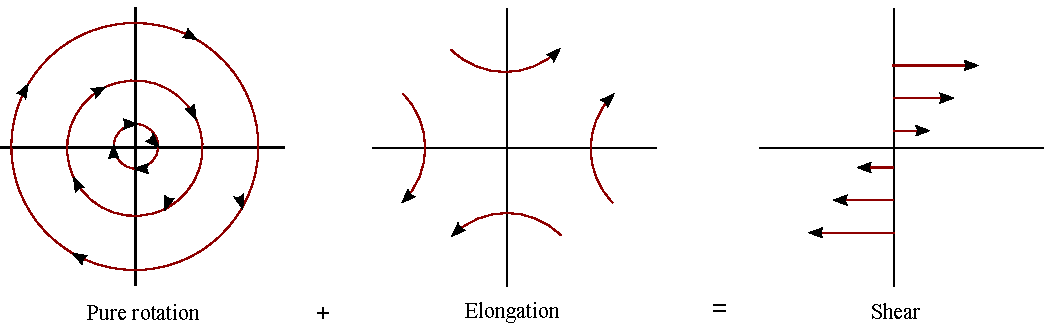
\includegraphics[width=1.2\textwidth]{figs/shear_decomposition}}
\begin{lpic}{figs/shear_decomposition(10cm,)}
   \lbl[b]{25,0;\vphantom{Hq}Rotation}
   \lbl[b]{85,0;\vphantom{Hq}stretching}
   \lbl[b]{152,0;\vphantom{Hq}shear}
   \lbl[c]{55,30;$+$}
   \lbl[c]{120,30;$=$}
   \lbl[b]{55,0;\vphantom{Hq}$+$}
   \lbl[b]{120,0;\vphantom{Hq}$=$}
\end{lpic}  
\end{center}
\caption{\label{fig:shear_decomposition} Decomposition of the simple shear flow into rotation and strain.}%
\end{figure}


\section{The Jeffery equation and its solutions}\seclab{jefferyequation}

In this section we consider axisymmetric particles: particles which are rotationally symmetric around an axis of symmetry. For such particles the orientational configuration may be represented by a unit vector $\ve n$, attached to the axis of symmetry. As alluded to in Sec.~\ref{sec:forces}, Jeffery presents two major results in his seminal paper from 1922 \cite{jeffery1922}. First, he calculates the hydrodynamic torque on a ellipsoid, not necessarily axisymmetric, in any linear flow. Second, he derives the equation of motion of an inertia-free, axisymmetric ellipsoid (a spheroid). This equation of motion is often referred to as the Jeffery equation. In our notation the Jeffery equation is
\begin{align}
	\dot{\ve n} &= \ma O \ve n + \Lambda \left(\ma S \ve n - \ve n \ve n \transpose \ma S \ve n\right).\eqnlab{jeffery}
\end{align}
Here $\ma O$ and $\ma S$ are the anti-symmetric and symmetric parts of the fluid gradient, as introduced in Sec.~\ref{sec:forces}. The parameter $\Lambda$ is a particle shape factor. For a spheroid of aspect ratio $\lambda$ the shape factor is
\begin{align*}
	\Lambda = \frac{\lambda^2-1}{\lambda^2+1}.
\end{align*}
For most conceivable particle shapes, $-1 < \Lambda < 1$. Negative $\Lambda$ correspond to flat, disk-shaped particles, while positive $\Lambda$ correspond to elongated, rod-like particles. It was shown by Bretherton \cite{bretherton1962} that, given the correct shape factor $\Lambda$, Jeffery's equation is valid not only for spheroids, but for any axisymmetric particle. He also showed that there are extreme cases where $|\Lambda|>1$. In this thesis we consider particles with $|\Lambda|<1$, like the spheroid.

 The equation of motion for an inertia-free particle is given by force and torque balance on the particle. Then the center-of-mass velocity equals the fluid velocity at the center-of-mass position, a condition called \emph{advection}. Jeffery's equation is the rotational analogue of center-of-mass advection. In Paper B, we demonstrate how to derive Jeffery's equation. We start from the hydrodynamic torque and Newton's equation of motion, and take the limit $\st\to 0$. See also Appendix~\secref{triaxial_equation} and the discussion in \Secref{experiment} for the generalisation to non-axisymmetric particles. In the following, we will instead consider the possible solutions of the Jeffery equation \eqnref{jeffery}.

Jeffery's equation is a non-linear vector equation, and as such it is seemingly hard to solve. However, the non-linearity is only apparent: it is due to the geometric constraint that $\ve n$ is a unit vector. The underlying dynamics is in fact linear. I will now explain two ways to understand this fact.

The vorticity $\ma O$ rotates $\ve n$, and the strain $\ma S$ aligns and stretches $\ve n$ towards its strongest eigendirection. The non-linear term $\ve n \ve n\transpose \ma S \ve n$ is simply the stretching component of the strain, which is subtracted in order to prevent elongation of $\ve n$. Bretherton (Sec.~6 in Ref.~\cite{bretherton1962}) realised that we may instead model the orientation of the particle with any vector $\ve q$ which obeys the same linear terms, but without compensating for any elongation:
\begin{align}
	\dot{\ve q} = \left(\ma O + \Lambda \ma S\right) \ve q.\eqnlab{jefferyq}
\end{align}
Owing to the common linear terms in \Eqnref{jeffery} and \Eqnref{jefferyq}, the vector $\ve q$ will have the same angular dynamics as $\ve n$. In addition, $\ve q$ may be stretched and compressed by the strain $\ma S$. But since we are only interested in the angular degrees of freedom, we can at any instant recover $\ve n$ by normalising $\ve q$ to unit length. Thus, the general solution of the Jeffery equation is given by solving \Eqnref{jefferyq} for $\ve q(t)$, then the solution to \Eqnref{jeffery} is given by normalising $\ve q(t)$ to unit length:
\begin{align}
	\ve n(t) &= \frac{\ve q(t)}{|\ve q(t)|}.\eqnlab{jefferysolution0}
\end{align}

Another, more mathematical, way of understanding how the linear companion equation \eqnref{jefferyq} arises is the following. Like above, we choose to represent the particle orientation by a vector $\ve q$ which is parallel to $\ve n$. Define $\ve q = \alpha(t)\ve n$, with $\alpha(t)$ an arbitrary function of time. We know from this definition that we may always recover $\ve n$ by normalising $\ve q$ to unit length. Now, we can calculate the equation of motion for $\ve q$:
\begin{align}
	\diff{\ve q}{t} &= \diff{}{t}\left(\alpha \ve n\right) \nn \\
	&= \dot \alpha \ve n + \alpha \dot{\ve n} \nn\\
	&= \dot \alpha \ve n + \alpha \left(\ma O \ve n + \Lambda \left(\ma S \ve n - \ve n \ve n \transpose \ma S \ve n\right)\right). \eqnlab{jefferyderivation1}
\end{align}
But $\alpha(t)$ is an arbitrary function which we may choose. In particular we can choose $\alpha(t)$ to be a function satisfying
\begin{align*}
	\dot \alpha &= \alpha \Lambda \ve n\transpose \ma S \ve n.
\end{align*}
By inserting this choice of $\alpha(t)$ into \Eqnref{jefferyderivation1}, we again arrive at \Eqnref{jefferyq}.

We will now consider the solutions of Jeffery's equation in time-independent flows. This case includes for example the simple shear flow, and indeed any linear flow. It is also a useful model when the flow changes only slowly in time, compared to the time it takes for the gradients to affect the particle orientation. First, I will describe the possible solutions of \Eqnref{jeffery} in linear flows. This picture is vital in understanding our argument in Paper C (see also \Secref{tumbling} in this thesis). Second, I will discuss the solutions of Jeffery's equation in a simple shear flow. The solutions are called the Jeffery orbits, and they play an important role in both Paper~A~and~B.

When $\ma O$ and $\ma S$ are time-independent the linear companion equation \eqnref{jefferyq} is solved by the matrix exponential:
\begin{align*}
		\ve q(t) = e^{(\ma O + \Lambda \ma S)t}\ve q(0).
\end{align*}
This solution implies that the long-time dynamics of $\ve q$, and therefore $\ve n$, is determined by the eigenvalues and eigenvectors of the matrix $\ma B = \ma O + \Lambda\ma S$. For an incompressible flow $\tr\ma B=0$, because $\tr\ma A=0$. In three spatial dimensions, the three eigenvalues of $\ma B$ must sum to zero. Thus, as noted by Bretherton \cite{bretherton1962}, there are three distinct possibilities for the eigensystem of $\ma B$:
\begin{enumerate}
	\item Three real eigenvalues, then
	\item[] $\ve q$ will align with the eigenvector corresponding to the largest eigenvalue.
	\item One real eigenvalue $a>0$, and a complex pair $-a/2 \pm i\omega$, then
	\item[] $\ve q$ will spiral into alignment with the eigenvector corresponding to the real eigenvalue.
	\item One real eigenvalue $a\leq0$, and a complex pair $-a/2 \pm i\omega$, then
	\item[] $\ve q$ will spiral out and finally rotate in the plane spanned by the real and imaginary parts of the complex eigenvector.
\end{enumerate}
\begin{figure}
\begin{center}
  \makebox[\textwidth]{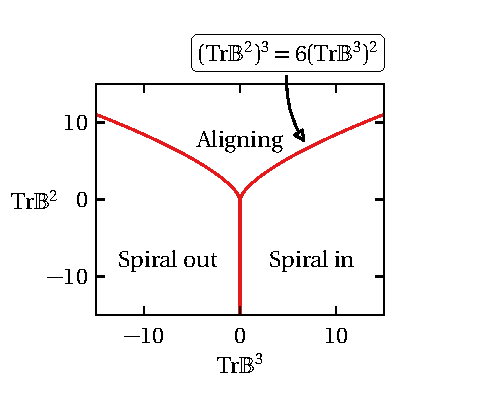
\includegraphics{figs/bmap}}
\end{center}
\caption{\label{fig:bmap}  Map of the three possible types of particle motion, as determined by the eigensystem of $\ma B=\ma O + \Lambda \ma S$.}%
\end{figure}
The characteristic equation for the eigenvalues $b$ of a $3\times3$-matrix $\ma B$ is
\begin{align*}
	-b^3 + b^2\tr \ma B  + \frac{b}{2}\left(\tr \ma B^2-(\tr \ma B)^2\right)+\det\ma B = 0.
\end{align*}
But for a traceless matrix $\tr \ma B=0$ and $\det \ma B = \tr\ma B^3/3$, because
\begin{align*}
	\tr \ma B &= b_1 + b_2 + b_3 = 0 \implies b_3 = -(b_1 + b_2),\\
	\intertext{therefore}
	\tr \ma B^3 &= b_1^3 + b_2^3 + b_3^3 = -3(b_1^2b_2 + b_1b_2^2),\\
	\det \ma B &= b_1b_2b_3 = -(b_1^2b_2 + b_1b_2^2).
\end{align*}
Thus the characteristic equation simplifies to
\begin{align}
	-b^3 + \frac{b}{2}\tr \ma B^2 +\frac{1}{3}\tr\ma B^3 = 0. \eqnlab{bcharacteristic}
\end{align}
It is possible to solve \Eqnref{bcharacteristic} exactly for the eigenvalues, but the important observation is that they are determined by only two parameters: $\tr \ma B^2$ and $\tr\ma B^3$. In Fig.~\ref{fig:bmap} I illustrate how the three cases outlined above correspond to different values of $\tr \ma B^2$ and $\tr\ma B^3$. The boundary curve of the region of three real eigenvalues is where the discriminant $\Delta$ of the characteristic equation is zero:
\begin{align*}
 	\Delta = \left(\tr \ma B^2\right)^3 - 6\left(\tr \ma B^3\right)^2 = 0.
 \end{align*} 
In the region where there is a pair of complex eigenvalues, the two cases of spiral in or out are separated by $\tr \ma B^3=0$. Now, what follows is one of the key observations in our argument in Paper C. For any given flow gradient, changing the particle from rod-like to disk-shaped (or vice versa) transforms $\tr \ma B^3\to-\tr\ma B^3$ and therefore change the qualitative dynamics from aligning to rotating (or vice versa). This transformation may be understood because
\begin{align*}
	\tr \ma B^3 = 3\Lambda \tr \ma O\ma O \ma S + \Lambda^3 \tr \ma S\ma S \ma S.
\end{align*}
The other combinations of $\ma S$ and $\ma O$ which could be expected to contribute, such as $\tr \ma O\ma O \ma O$, vanish identically because of symmetries of $\ma O$ and $\ma S$. As explained above, changing a particle from rod-like to disk-shaped implies a change of sign of the shape factor $\Lambda$. The implications of this observation for the tumbling of particles in turbulent and random flows are further discussed in Sec.~\ref{sec:tumbling} in Part~II, and in Paper C. 

The remainder of this section concerns the case of simple shear flow. This case is characterised by $\tr \ma B^3=0$ and $\tr \ma B^2<0$. The simple shear has a special position among flows, and we understand the significance of the condition $\tr\ma B^3=0$ from the above discussion. First, a change of particle shape does not change the qualitative dynamics. Both disk-shaped particles and rod-like particles rotate in a shear flow. Second, $\ma B$ has a zero eigenvalue, as seen from the characteristic equation \eqnref{bcharacteristic}. The zero eigenvalue is important, because it implies that the particle dynamics never forgets its initial condition. The eigenvector of the zero eigenvalue is the vorticity direction\footnote{See Fig.~\ref{fig:coordinates} and Sec.~\ref{sec:shearflow} for the definition of the coordinate system and the terminology of its directions in a simple shear flow.}, thus the component of $\ve q$ in the vorticity direction is constant in a shear flow. The other two eigenvalues are an imaginary pair, resulting in a periodic rotation of $\ve q$.

In summary, the dynamics of $\ve q$ in a simple shear flow is a periodic rotation in a plane. The plane is normal to the vorticity direction, and determined by the initial condition of $\ve q$.

\begin{figure}
	\begin{center}
	  \makebox[\textwidth]{%
        \begin{subfigure}[b]{0.62\textwidth}
                \centering
                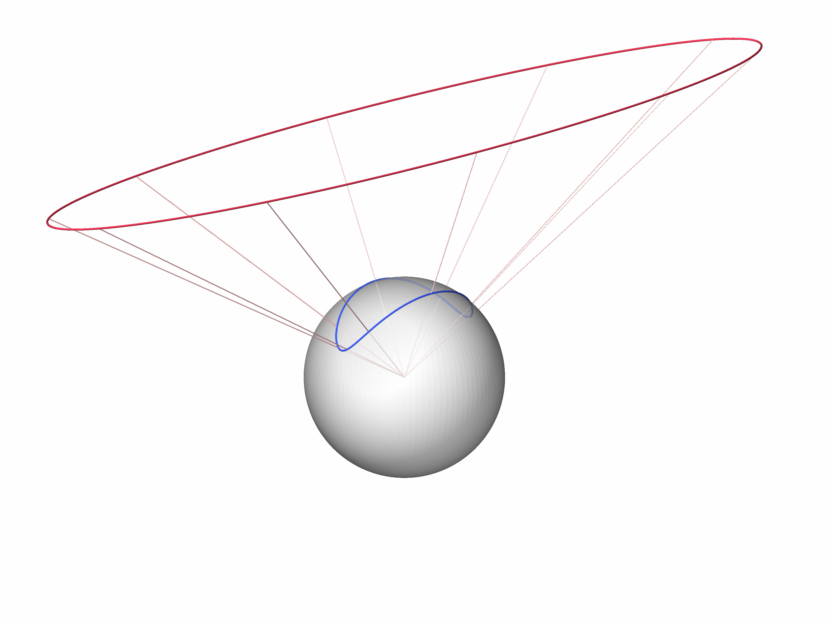
\includegraphics[width=\textwidth]{figs/projection_orbit1.png}
                \caption{}
                \label{fig:projection_orbit1}
        \end{subfigure}%
        \begin{subfigure}[b]{0.62\textwidth}
                \centering
                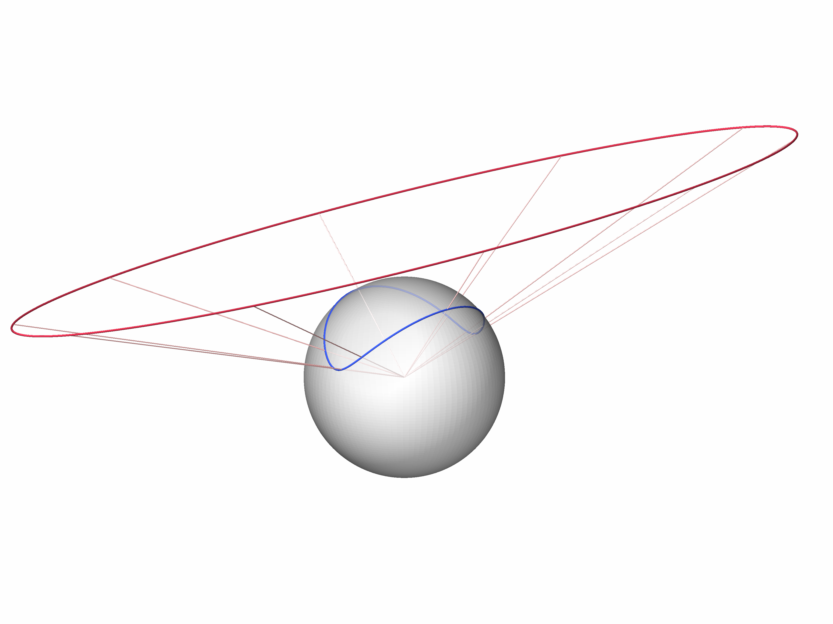
\includegraphics[width=\textwidth]{figs/projection_orbit2.png}
                \caption{}
                \label{fig:projection_orbit2}
        \end{subfigure}
        }
        \makebox[\textwidth]{%
        \begin{subfigure}[b]{0.62\textwidth}
                \centering
                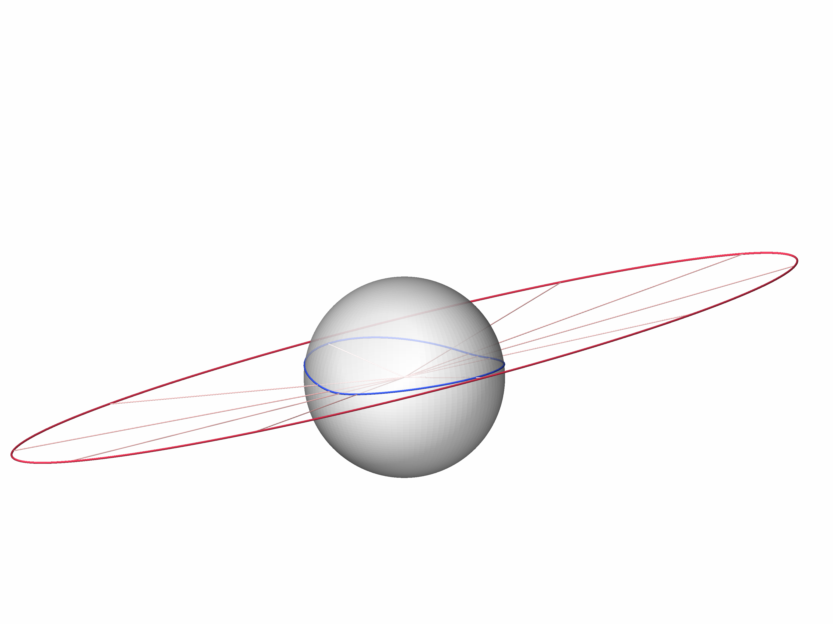
\includegraphics[width=\textwidth]{figs/projection_orbit3.png}
                \caption{}
                \label{fig:projection_orbit3}
        \end{subfigure}
        \begin{subfigure}[b]{0.62\textwidth}
                \centering
                %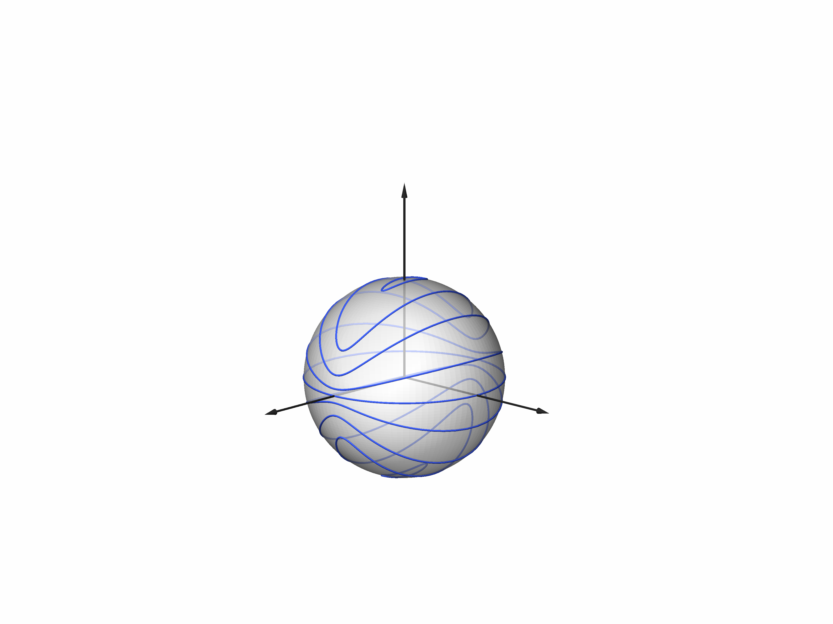
\includegraphics[width=\textwidth]{figs/projection_orbit4.png}
				\begin{lpic}{figs/projection_orbit4(7cm,)}
				   \lbl[tl]{60,55;$\hat{\ve x}$}
				   \lbl[tl]{150,55;$\hat{\ve y}$}
				   \lbl[tl]{105,130;$\hat{\ve z}$}
				\end{lpic}
                \caption{}
                \label{fig:projection_orbit4}
        \end{subfigure}        
	  }%
	\end{center}
    \caption{\textbf{(a-c)} Illustrations of how the trajectories $\ve q(t)$ (red) produces the Jeffery orbits $\ve n(t)$ (blue) upon projection onto the unit sphere. \textbf{(d)} Sample of resulting Jeffery orbits with coordinate system. All trajectories correspond to a particle of aspect ratio $\lambda=5$ in a simple shear flow.}\label{fig:projection_orbits}
\end{figure}


When the trajectories $\ve q(t)$ are projected onto the unit sphere, the result $\ve n(t)$ are the Jeffery orbits. I visualise this in Fig.~\ref{fig:projection_orbits} where the trajectories $\ve q(t)$ and $\ve n(t)$ are shown for three different initial conditions.

The solutions to Jeffery's equation in a simple shear flow are degenerate: the orientational trajectory depends on the initial condition indefinitely. In many realistic situations this long-time memory hardly seems plausible. The degeneracy is a result of the assumptions made in the course deriving the Jeffery orbits. Each assumption corresponds to a physical mechanism, and in order to understand how the degenaracy may be broken these mechanisms must be investigated. The three assumptions we believe most important to investigate are the following.

First, the particle may not be axisymmetric. In this case the dynamics is more complicated, but still depends on the initial conditions indefinitely. Tri-axial particles are discussed further in relation to Paper A in Sec.~\ref{sec:experiment}.

Second, there may be inertial effects. Fluid inertia was neglected when we used the resistance tensor formulation \eqnref{resistanceformulation} for the torque on a particle. Particle inertia was neglected when Newton's equation reduced to Jeffery's equation in the advective limit $\st \to 0$. In Paper B we describe how the effects of a small amount of particle inertia break the degeneracy of the solutions $\ve n(t)$. See the discussion in \Secref{inertia} for an outlook on the case of fluid inertia.

Finally, the third mechanism is Brownian noise. The idea is that thermal fluctuations kick the particle out of one Jeffery orbit and into another. After some time, the initial condition is forgotten and the state of the particle is described by an orientational probability distribution. The problem of computing the orientational distribution has a long history, and in the next Section I briefly review some of the methods and results.

\section{Orientational distributions}\seclab{orientationaldistributions}

In this Section we consider the orientational dynamics of an axisymmetric particle, represented by the vector $\ve n$. In this case the orientational distribution is a function $P(\ve n, t)$ which describes the probability of observing the particle with orientation\footnote{Strictly, $P(\ve n, t)\rd S$ is the probability to find $\ve n$ on the surface element $\rd S$ at time $t$.} $\ve n$ at time $t$. Instead of asking for the orientational trajectory $\ve n(t)$ of a particle given the initial condition $\ve n(0)$, we now ask what the orientational distribution $P(\ve n, t)$ is, given the initial condition $P(\ve n, 0)$.

The by far most common approach is to consider a diffusion equation for the unit vector $\ve n$. My view of the diffusion approximation is the following. The orientation of the particle is driven by very many, very small and very fast kicks. In the case of particles in fluids, the small kicks originate in the bombardment of fluid molecules onto the particle surface. These \emph{microscopic} kicks are so small and fast that we never see them directly. But after a short time, enough kicks have accumulated into an observable change. If we reset the particle orientation and start over, the microscopic kicks will again accumulate into an observable change. But because the molecular bombardment is not exactly the same every time, the accumulated change is different every time. The ``diffusion approximation'' is to not consider all the details of the random kicks, but to only consider the \emph{mean value} and \emph{variance} of the accumulated changes. The idea is to replace the complicated accumulation of microscopic kicks with randomly chosen changes. The randomly chosen steps will have the correct mean value and variance, but all other details are neglected. The idea is based mathematically in the ``Central Limit Theorem'' of statistics, stating that if you add many random numbers the sum will converge to be normally distributed (under certain conditions). For a complete and very readable account of the method I point to the book \emph{Stochastic Processes in Physics and Chemistry}, by van Kampen \cite{kampen2007}.

The governing equation for the orientational distribution of an axisymmetric particle in the diffusion approximation is the Fokker-Planck equation
\begin{align}
	\frac{\partial}{\partial t}P(\ve n, t) &= -\frac{\partial}{\partial \ve n}\left[\ve J (\ve n, t)P(\ve n, t)\right] + \mathcal D \frac{\partial^2}{\partial \ve n^2}P(\ve n, t).\eqnlab{fpejeff}
\end{align}
The first term on the right hand side is referred to as the drift, and the second as the diffusion. The drift is due to the deterministic fluid flow, and $\ve J(\ve n, t)$ represents the right hand side of the Jeffery equation \eqnref{jeffery}. The diffusion term is due to the random kicks, and $\mathcal D$ is the rotational diffusion constant. Since $\ve n$ is a unit vector, the Fokker-Planck equation is defined on the unit sphere. Therefore the derivative with respect to $\ve n$ is defined as $\partial/\partial_{\ve n} = (\ma I-\ve n\ve n\transpose)\nabla$, with $\nabla$ the usual gradient in $\mathbb R^3$. In Appendix~\secref{fpesphere} I explain this in more detail, and present a full derivation of \Eqnref{fpejeff}. 

For the purposes of this thesis, and more specifically Paper B, we consider the case when a particle is suspended in a simple shear flow, and at the same time is subject to Brownian noise. As mentioned in the \Secref{jefferyequation}, the solutions to Jeffery's equation in a simple shear flow are degenerate. The orientational distribution of $\ve n$ under the influence of, for example, thermal noise has been extensively studied, as a means of explaining how particles in shear ``forget'' their initial conditions. A thorough review is given in \cite{brenner1974}, and what follows is a brief summary.

The dynamics is governed by a single dimensionless parameter, the P\'eclet number $\pe = s/\mathcal D$. Here $\mathcal D$ is the diffusion constant in \Eqnref{fpejeff}, and $s$ is the shear strength, or the strength of the drift term in \Eqnref{fpejeff}. A small value of $\pe$ means that the noise is strong, and vice versa. 

\begin{figure}
\begin{center}
  \makebox[\textwidth]{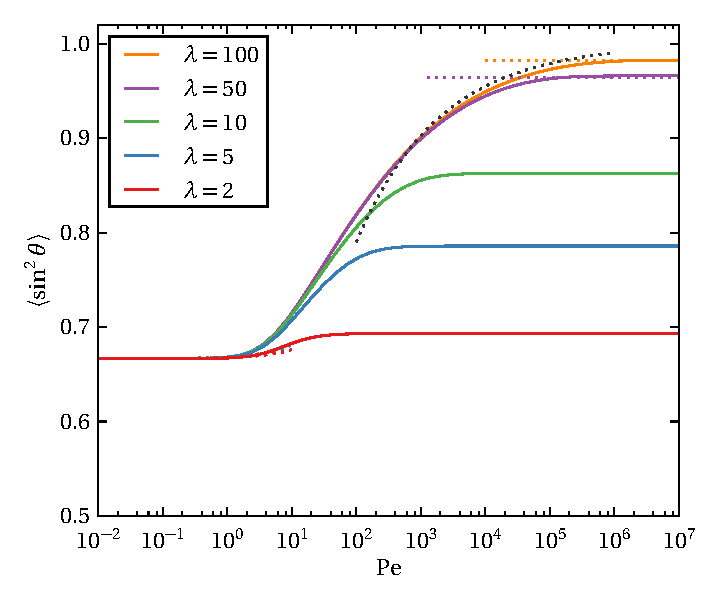
\includegraphics{figs/sintheta1.pdf}}
\end{center}
\caption{\figlab{sintheta1} Stationary average $\langle \sin ^2\theta \rangle$ for an axisymmetric particle in a shear flow subject to random noise, shown as function of the P\'eclet number $\pe = s/\mathcal D$ for different values of the particle aspect ratio $\lambda$. Larger $\pe$ corresponds to less noise. Solid lines are numerical solutions. Dotted lines show asymptotes in regimes of weak and intermediate noise, given by Eqs.~(9.5) and (9.13a) with (9.15) in \cite{brenner1974}.}%
\end{figure}

For small $\pe$, when the noise dominates, the orientational distribution is uniform -- all orientations are equally likely. When the noise is decreased, the orientational distribution begins to reflect the Jeffery orbits. As $\pe$ becomes larger and the shear grows increasingly important, the probability of seeing a particle aligned with the flow direction increases. 
But surprisingly, when $\pe$ becomes large enough, the stationary orientational distribution converges and becomes \emph{independent of} $\pe$. In other words, when the noise is small enough, the particles follow the Jeffery orbits, but every now and then jump to a different orbit.

The stationary orientational distribution in general depends on the value of $\pe$ and the particle aspect ratio $\lambda$. In order to quantify the above discussion, I show numerical solutions\footnote{The details of how I solve \Eqnref{fpejeff} numerically can be found in Appendix~\ref{app:fpe_sphere}.} for the stationary average $\langle \sin^2\theta \rangle$ in \Figref{sintheta1}. The angle $\theta$ is the polar angle of $\ve n$, such that $n_z = \cos\theta$. It is also the angle to the vorticity direction, see \Figref{coordinates}.

For small $\pe$ we see that $\langle \sin^2\theta \rangle = 2/3$, the expected value for a uniformly random distribution. But for large $\pe$, the average reaches a plateau, depending on particle aspect ratio $\lambda$. The asymptotic solutions of \Eqnref{fpejeff} described in \cite{brenner1974} are shown as dotted lines. In particular, Hinch \& Leal \cite{hinch1972} solved the case of weak noise, that is large $\pe$. They obtained an expression for the height of the plateau valid for thin particles, $\lambda\gg1$. The numerical solution confirms their prediction.

In Paper B we compute the same orientational average, $\langle \sin^2\theta \rangle$, when the particle has a small but finite mass, as characterised by the Stokes number.



\end{document}
